% $Header: /home/vedranm/bitbucket/beamer/solutions/conference-talks/conference-ornate-20min.de.tex,v 90e850259b8b 2007/01/28 20:48:30 tantau $

\documentclass{beamer}

\mode<presentation>{
  \usetheme{Warsaw}
  \setbeamercovered{transparent}}

\usepackage[latin1]{inputenc}
\usepackage{times}
\usepackage[T1]{fontenc}
\usepackage{graphicx}
\usepackage{hyperref}
\usepackage{pdfpages}

\usepackage{tikz}
\usepackage{xcolor}
\usepackage{pdfpages}
\usepackage{courier}

\bibliographystyle{apalike}

\definecolor{olive}{rgb}{0.3, 0.4, .1}
\definecolor{fore}{RGB}{249,242,215}
\definecolor{back}{RGB}{51,51,51}
\definecolor{title}{RGB}{255,0,90}
\definecolor{dgreen}{rgb}{0.,0.6,0.}
\definecolor{gold}{rgb}{1.,0.84,0.}
\definecolor{gold2}{rgb}{1.,0.6,0.}
\definecolor{JungleGreen}{cmyk}{0.99,0,0.52,0}
\definecolor{bluegreen}{cmyk}{0.85,0,0.33,0}
\definecolor{rawsienna}{cmyk}{0,0.72,1,0.45}
\definecolor{magenta}{cmyk}{0,1,0,0}

\definecolor{light-gray}{gray}{0.95}
\definecolor{dark-gray}{gray}{0.1}

\definecolor{fore}{RGB}{249,242,215}
\definecolor{back}{RGB}{51,51,51}
\definecolor{title}{RGB}{255,0,90}

%\usecolortheme{albatross}
%\usetheme{default}
%\beamertemplatenavigationsymbolsempty


%\setbeamercolor{titlelike}{fg=title}
%\setbeamercolor{normal text}{fg=fore,bg=back}

\newcommand\Fontvi{\fontsize{6}{8}\selectfont}
\newcommand\Fontviii{\fontsize{8}{10}\selectfont}


\date{\textcolor{light-gray}{\today}}


\AtBeginSubsection[]{
  \begin{frame}<beamer>{Contents}
    \tableofcontents[currentsection,currentsubsection]
  \end{frame}}


\begin{document}

\usebackgroundtemplate{
\tikz\node[opacity=.5] {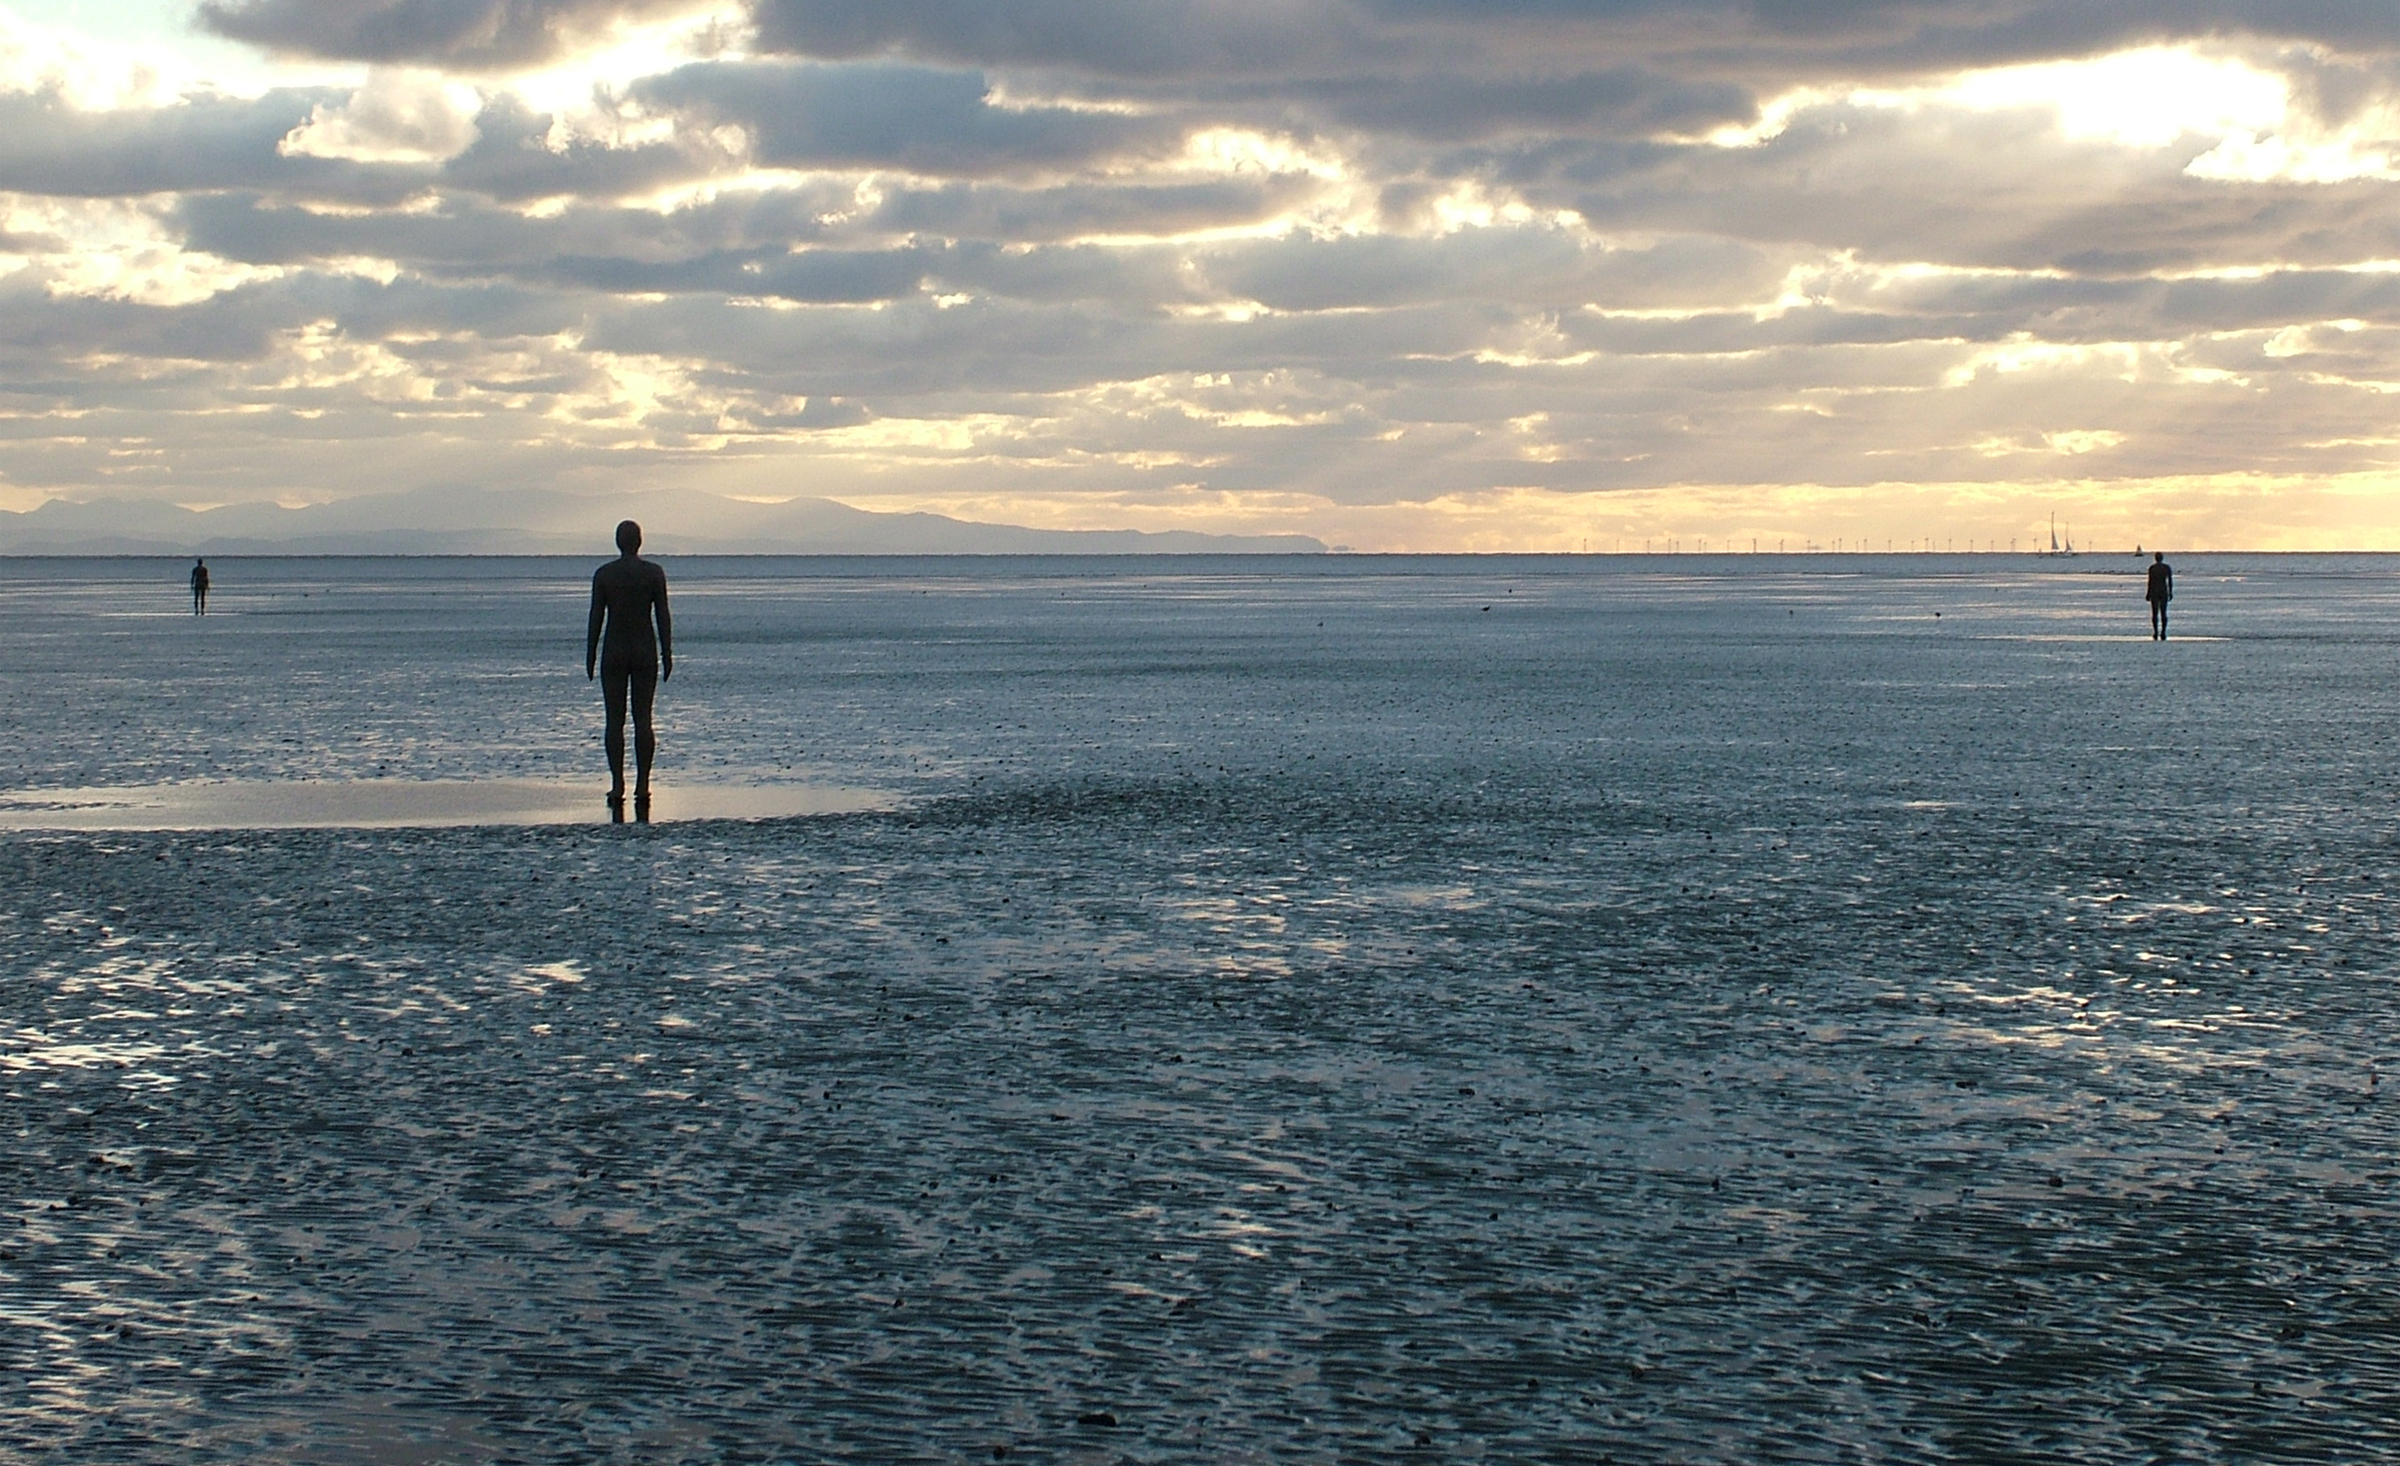
\includegraphics[height=8.67cm,width=12.587cm]{Another_Place3_edit2.jpg}};}

\title{Assessing Harvest Control Rules (HCRs)}

\subtitle{Management Strategy Evaluation (MSE)}

\date{SWGSM Barcelona \\ ~ \\ May $25^{th}$ 2014}

\setkeys{Gin}{width=0.75\textwidth}
%\logo{
\includegraphics[height=0.8cm, width=2.22cm]{logoICCAT-2.jpg}}
        
\author{\parbox[t]{4.0cm}{\center Laurence Kell \\ ICCAT Secretariat}}
    
\AtBeginSubsection[]{
 \begin{frame}<beamer>{Contents}
    \tableofcontents[currentsection,currentsubsection]
 \end{frame}}

\begin{frame} \titlepage \end{frame}

%http://www.fao.org/fishery/topic/13302/en

\begin{frame}\textcolor{blue}{\large{\textbf{Outline}}} \tableofcontents \end{frame}

\section{Precautionary Approach}
\begin{frame}\frametitle{Precautionary Approach} 
  \smallskip\textbf{When managing fisheries decisions have to be made with incomplete knowledge}\smallskip
  \Fontviii
  \begin{itemize} %[<+->]
     \item Undesirable outcomes should be be anticipated; measures taken to reduce the risk of them occurring; corrective measures should be applied immediately and be effective within an acceptable time frame. 
     \item Requires \textbf{L}imit and \textbf{t}hreshold \textbf{R}eference \textbf{P}oints, used as part of a \textbf{H}arvest \textbf{Control} \textbf{Rule}, 
     \item Consideration must be given to major uncertainties. e.g. \\ in status of the stocks relative to reference points, biology, environmental events, ...
    \end{itemize}
\end{frame}

    
\begin{frame}\frametitle{Precautionary Approach} 
  \smallskip Harvest Control Rules\smallskip\\
  \Fontviii
  \begin{itemize} %[<+->]
    \item \textbf{HCR}s will not necessarily be precautionary if they are not formally evaluated to determine how well they actually achieve their goals given uncertainty.
    \item There use simulation first to evaluate the impact of the main sources of uncertainty on the robustness of alternative \textbf{HCR}s and Management Strategies
  \end{itemize}
\end{frame}

\begin{frame}\frametitle{Management Strategy Evaluation} 
  \smallskip\textbf{Simulation modelling to evaluate the impact of uncertainty and reducing the risk of doing something stupid}\smallskip 
  \Fontviii
  \begin{itemize} %[<+->]
     \item Allows a fuller consideration of uncertainty as required by the Precautionary Approach; 
     \item Provides stability if management objectives and how to evaluate how well alternative  
	   management strategies meet them are agreed through a dialogue between scientists and stakeholders; and 
     \item Can be used to guide the scientific process by identifying where the reduction of scientific 
	   uncertainty will improve management and so help to ensure that expenditure is prioritised to provide 
	   the best research, monitoring and enforcement. 
  \end{itemize}
\end{frame}


\section{Process}
\begin{frame}\frametitle{MSE Process} 
  \smallskip\textbf{Six Step Program}\smallskip
  \Fontviii
  \begin{description}%[<+->]
    \item[Identification] of management objectives and mapping these to performance measures to quantify how well they are achieved\
    \item[Selection] of hypotheses about system dynamics for building \textbf{O}perating \textbf{M}odels (i.e. Simulation Models)
    \item[Building] the simulation models, i.e. Conditioning them on data and knowledge, and rejecting and weighting different hypotheses.
    \item[Identifying] alternative management strategies, (i.e.the combination of pre-defined data, stock assessment methods, reference points and HCRs.
    \item[Running] the simulations using the HCRs as feedback control procedures; and
    \item[Agreeing] the Management Strategies that best meet management objectives.
 \end{description}
 \end{frame}


\section{Examples}

\begin{frame}{Principles of Decision Making [REC 11-13]}
   \smallskip\textbf{Red Quadrant} i.e. overfished and overfishing\smallskip\\
  \begin{columns}[t] % contents are top vertically aligned
   \begin{column}[T]{5cm} % alternative top-align that's better for graphics
    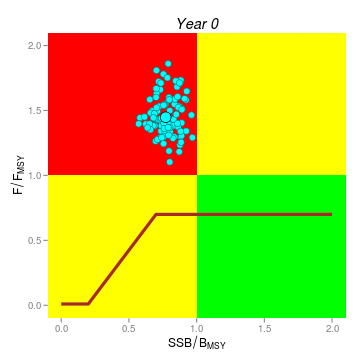
\includegraphics[height=40mm]{hcrI1.png}
   \end{column}
   \begin{column}[T]{6cm} % each column can also be its own environment
   \Fontviii
   \begin{itemize}%[<+->]
       \item Management should ensure a high probability of ending overfishing in as \textbf{short a time period as possible}
       \item A plan must be adopted for rebuilding taking into account stock biology and SCRS advice
       \item Risk Levels, Probabilities and Time Scales?
       \item Short-term objective to stop overfishing,
       \item Long-term objective to recover stock to a level that can support MSY
   \end{itemize}
   \end{column}
\end{columns}
\end{frame}
     
\begin{frame}\frametitle{Principles of Decision Making [REC 11-13]} \smallskip\textbf{Stop Overfishing}\smallskip\\ 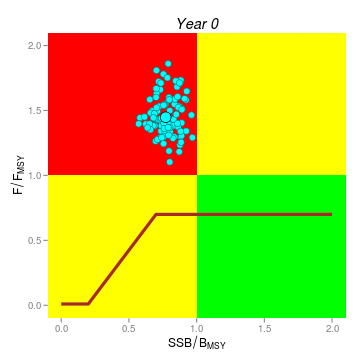
\includegraphics[height=50mm,width=50mm]{hcrI1.png}\end{frame}
\begin{frame}\frametitle{Principles of Decision Making [REC 11-13]} \smallskip\textbf{Stop Overfishing}\smallskip\\ 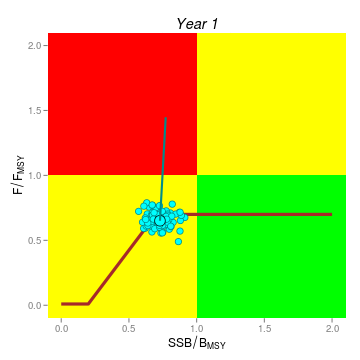
\includegraphics[height=50mm,width=50mm]{hcrI2.png}\end{frame}
\begin{frame}\frametitle{Principles of Decision Making [REC 11-13]} \smallskip\textbf{Stop Overfishing}\smallskip\\ 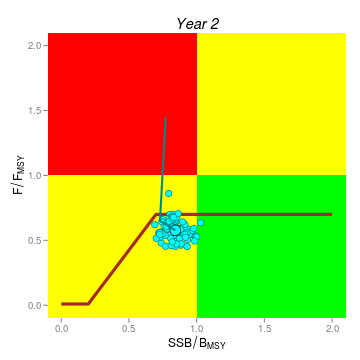
\includegraphics[height=50mm,width=50mm]{hcrI3.png}\end{frame}
\begin{frame}\frametitle{Principles of Decision Making [REC 11-13]} \smallskip\textbf{Stop Overfishing}\smallskip\\ 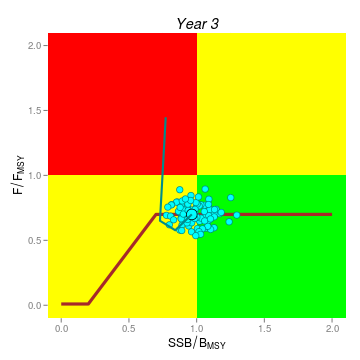
\includegraphics[height=50mm,width=50mm]{hcrI4.png}\end{frame}
\begin{frame}\frametitle{Principles of Decision Making [REC 11-13]} \smallskip\textbf{Stop Overfishing}\smallskip\\ 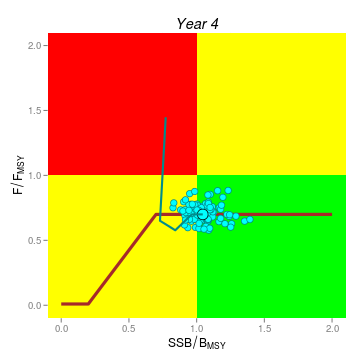
\includegraphics[height=50mm,width=50mm]{hcrI5.png}\end{frame}
\begin{frame}\frametitle{Principles of Decision Making [REC 11-13]} \smallskip\textbf{Stop Overfishing}\smallskip\\ 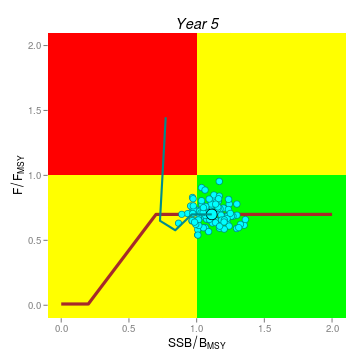
\includegraphics[height=50mm,width=50mm]{hcrI6.png}\end{frame}
\begin{frame}\frametitle{Principles of Decision Making [REC 11-13]} \smallskip\textbf{Stop Overfishing}\smallskip\\ 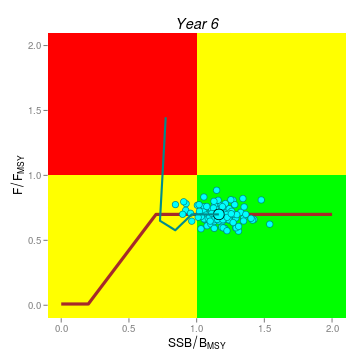
\includegraphics[height=50mm,width=50mm]{hcrI7.png}\end{frame}
\begin{frame}\frametitle{Principles of Decision Making [REC 11-13]} \smallskip\textbf{Stop Overfishing}\smallskip\\ 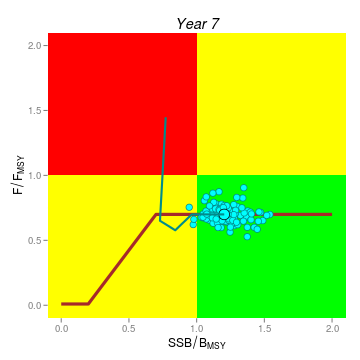
\includegraphics[height=50mm,width=50mm]{hcrI8.png}\end{frame}
\begin{frame}\frametitle{Principles of Decision Making [REC 11-13]} \smallskip\textbf{Stop Overfishing}\smallskip\\ 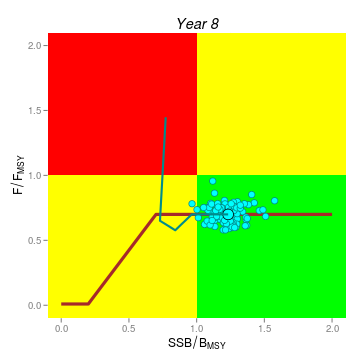
\includegraphics[height=50mm,width=50mm]{hcrI9.png}\end{frame}
%\begin{frame}\frametitle{Principles of Decision Making [REC 11-13]} \smallskip\textbf{Stop Overfishing}\smallskip\\ 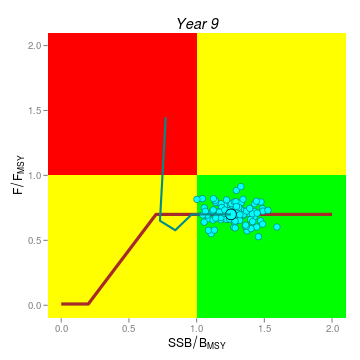
\includegraphics[height=50mm,width=50mm]{hcrI10.png}\end{frame}
%\begin{frame}\frametitle{Principles of Decision Making [REC 11-13]} \smallskip\textbf{Stop Overfishing}\smallskip\\ 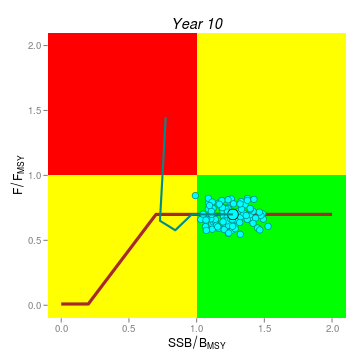
\includegraphics[height=50mm,width=50mm]{hcrI11.png}\end{frame}
%\begin{frame}\frametitle{Principles of Decision Making [REC 11-13]} \smallskip\textbf{Stop Overfishing}\smallskip\\ 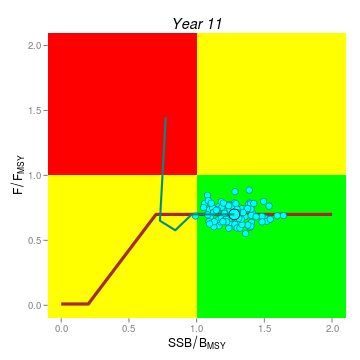
\includegraphics[height=50mm,width=50mm]{hcrI12.png}\end{frame}



\begin{frame}{Principles of Decision Making [REC 11-13]}
   \smallskip\textbf{Short a time as possible?}\smallskip\\
  \begin{columns}[t] % contents are top vertically aligned
   \begin{column}[T]{5cm} % alternative top-align that's better for graphics
    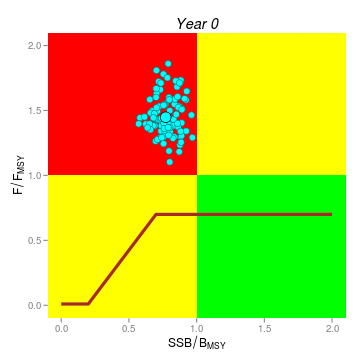
\includegraphics[height=40mm]{hcrI1.png}
   \end{column}
   \begin{column}[T]{6cm} % each column can also be its own environment
   \smallskip Trade-offs between objectives\smallskip\\
   \Fontviii
   \begin{description}%[<+->]
       \item[Short-term] objective to stop overfishing,
       \item[Long-term] objective to recover stock to a level that can support MSY
     \end{description}
   \end{column}
\end{columns}
\end{frame}
\begin{frame}\frametitle{Principles of Decision Making [REC 11-13]} \smallskip\textbf{Acceptable Time Frame?}\smallskip\\ 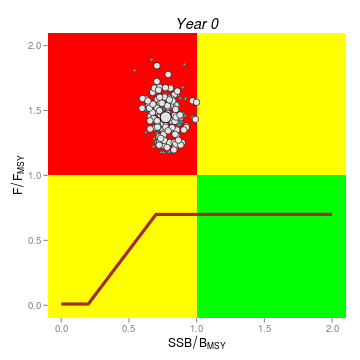
\includegraphics[height=50mm,width=50mm]{hcrII1.png}\end{frame}
\begin{frame}\frametitle{Principles of Decision Making [REC 11-13]} \smallskip\textbf{Acceptable Time Frame?}\smallskip\\ 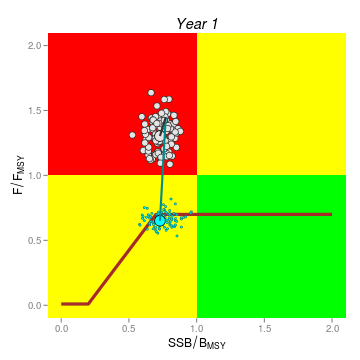
\includegraphics[height=50mm,width=50mm]{hcrII2.png}\end{frame}
\begin{frame}\frametitle{Principles of Decision Making [REC 11-13]} \smallskip\textbf{Acceptable Time Frame?}\smallskip\\ 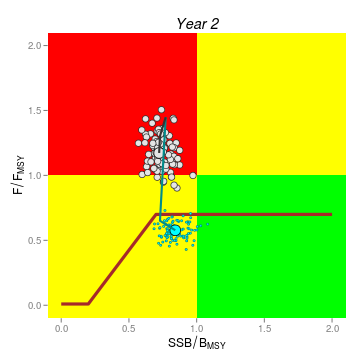
\includegraphics[height=50mm,width=50mm]{hcrII3.png}\end{frame}
\begin{frame}\frametitle{Principles of Decision Making [REC 11-13]} \smallskip\textbf{Acceptable Time Frame?}\smallskip\\ 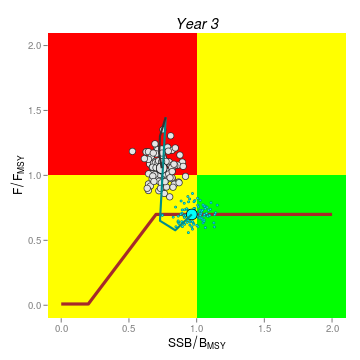
\includegraphics[height=50mm,width=50mm]{hcrII4.png}\end{frame}
\begin{frame}\frametitle{Principles of Decision Making [REC 11-13]} \smallskip\textbf{Acceptable Time Frame?}\smallskip\\ 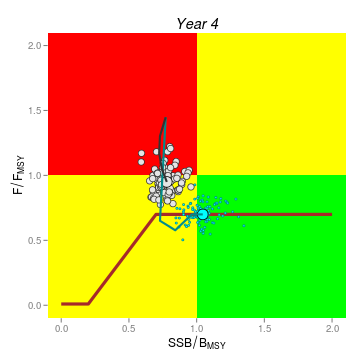
\includegraphics[height=50mm,width=50mm]{hcrII5.png}\end{frame}
\begin{frame}\frametitle{Principles of Decision Making [REC 11-13]} \smallskip\textbf{Acceptable Time Frame?}\smallskip\\ 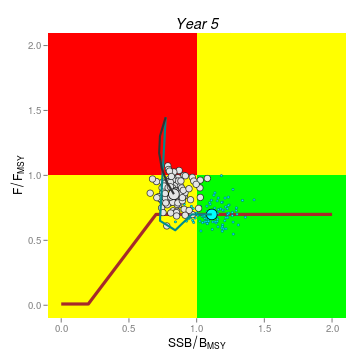
\includegraphics[height=50mm,width=50mm]{hcrII6.png}\end{frame}
\begin{frame}\frametitle{Principles of Decision Making [REC 11-13]} \smallskip\textbf{Acceptable Time Frame?}\smallskip\\ 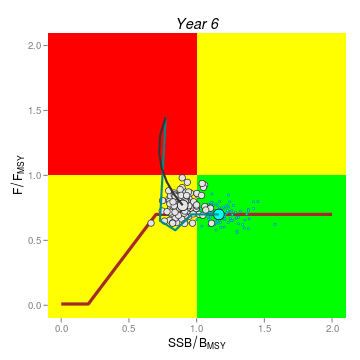
\includegraphics[height=50mm,width=50mm]{hcrII7.png}\end{frame}
\begin{frame}\frametitle{Principles of Decision Making [REC 11-13]} \smallskip\textbf{Acceptable Time Frame?}\smallskip\\ 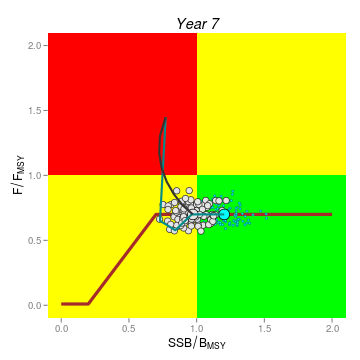
\includegraphics[height=50mm,width=50mm]{hcrII8.png}\end{frame}
\begin{frame}\frametitle{Principles of Decision Making [REC 11-13]} \smallskip\textbf{Acceptable Time Frame?}\smallskip\\ 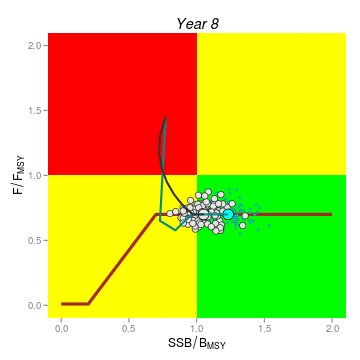
\includegraphics[height=50mm,width=50mm]{hcrII9.png}\end{frame}
\begin{frame}\frametitle{Principles of Decision Making [REC 11-13]} \smallskip\textbf{Acceptable Time Frame?}\smallskip\\ 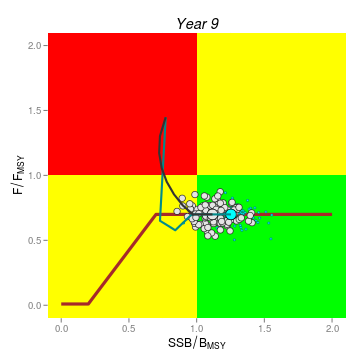
\includegraphics[height=50mm,width=50mm]{hcrII10.png}\end{frame}
\begin{frame}\frametitle{Principles of Decision Making [REC 11-13]} \smallskip\textbf{Acceptable Time Frame?}\smallskip\\ 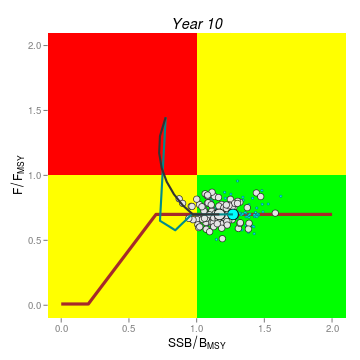
\includegraphics[height=50mm,width=50mm]{hcrII11.png}\end{frame}
\begin{frame}\frametitle{Principles of Decision Making [REC 11-13]} \smallskip\textbf{Acceptable Time Frame?}\smallskip\\ 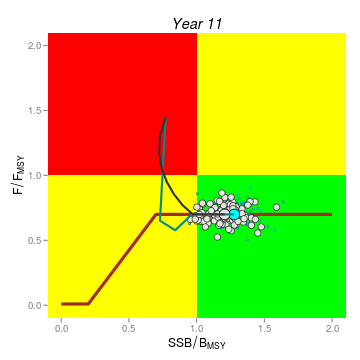
\includegraphics[height=50mm,width=50mm]{hcrII12.png}\end{frame}



\begin{frame}\frametitle{Principles of Decision Making [REC 11-13]} \smallskip\textbf{How Do The Recoveries Compare?}\smallskip\\ 
\begin{columns}[t] 
\begin{column}[T]{6cm}
  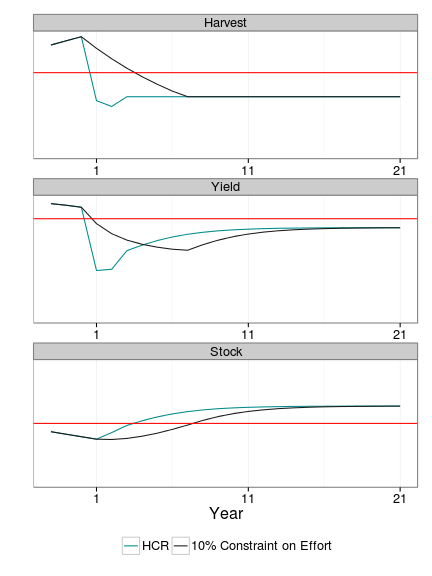
\includegraphics[height=50mm,width=50mm]{hcr-ts.png}
\end{column}
\begin{column}[T]{4cm} % each column can also be its own environment
     \smallskip\textbf{10\% F Constraint}\smallskip\\
       \Fontviii
       \begin{itemize}%[<+->]
          \item Takes 7 years for F to be reduced to target
          \item Yield is higher initially but is less in the medium term
          \item Stock recovery takes twice as long, 6 as opposed to 3 years
        \end{itemize}
\end{column}
\end{columns}    
\end{frame}

\begin{frame}{Principles of Decision Making [REC 11-13]}
     \smallskip\textbf{Green Quadrant} Stock Recovered\smallskip\\
     \begin{columns}[t] % contents are top vertically aligned
     \begin{column}[T]{5cm} % alternative top-align that's better for graphics
          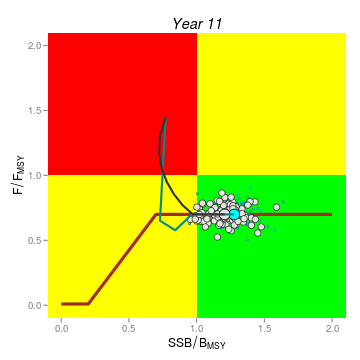
\includegraphics[height=40mm]{hcrII12.png}
     \end{column}
     \begin{column}[T]{5cm} % each column can also be its own environment
                  \Fontviii
                  \begin{itemize}
                  \item Management measures shall be designed to result in a high probability of maintaining the stock within the green quadrant
                 \end{itemize}        
     \end{column}
     \end{columns}    
\end{frame}


\begin{frame}{MSE Example}
      \smallskip\textbf{MSE Example}\smallskip\\
     \begin{columns}[t] % contents are top vertically aligned
     \begin{column}[T]{5cm} % alternative top-align that's better for graphics
        \smallskip\textbf{Finance} Invest the Capital and live off Interest\smallskip\\
        \Fontviii
       \begin{itemize}
         \item Get a bank statement as required
         \item {\color{red} Warning!} Investments can decrease as well as increase in value 
       \end{itemize}        
     \end{column}
     \begin{column}[T]{5cm} % each column can also be its own environment
      \smallskip\textbf{Fisheries} Keep the stock above $B_{MSY}$ and harvest the surplus\smallskip\\
       \Fontviii
       \begin{itemize}[<+->]
         \item Only get a stock assessment once a year, if lucky!
         \item Estimate of current stock status has large uncertainty  
         \item What if environmental change recruitment? 
       \end{itemize}        
     \end{column}
     \end{columns}    
\end{frame}


\begin{frame}\frametitle{MSE Example} \smallskip\textbf{There has been a {\color{blue} Regime Shift}}\smallskip\\ Is it A or B? 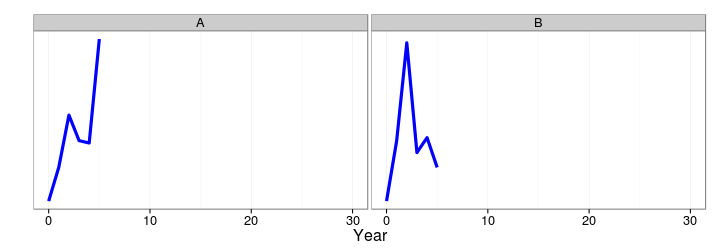
\includegraphics[height=25mm,width=100mm]{doug1.png}\end{frame}
%\begin{frame}\frametitle{MSE Example} \smallskip\textbf{There has been a {\color{blue} Regime Shift}}\smallskip\\ Is it A or B? 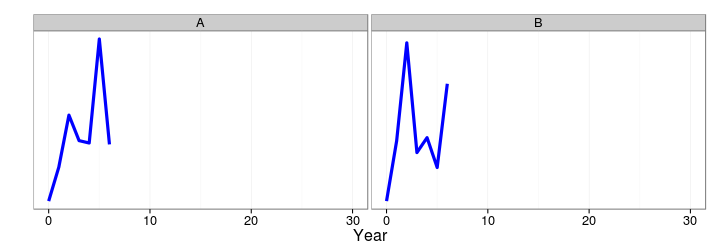
\includegraphics[height=25mm,width=100mm]{doug2.png}\end{frame}
%\begin{frame}\frametitle{MSE Example} \smallskip\textbf{There has been a {\color{blue} Regime Shift}}\smallskip\\ Is it A or B? 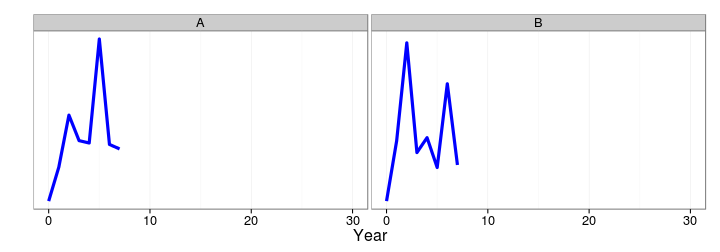
\includegraphics[height=25mm,width=100mm]{doug3.png}\end{frame}
\begin{frame}\frametitle{MSE Example} \smallskip\textbf{There has been a {\color{blue} Regime Shift}}\smallskip\\ Is it A or B? 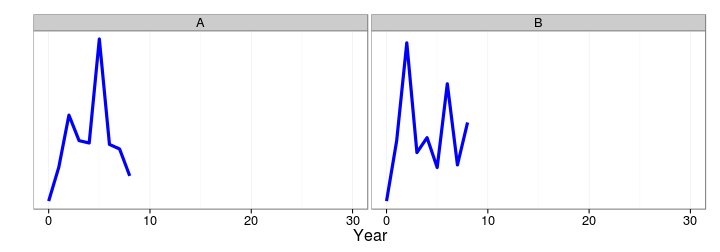
\includegraphics[height=25mm,width=100mm]{doug4.png}\end{frame}
%\begin{frame}\frametitle{MSE Example} \smallskip\textbf{There has been a {\color{blue} Regime Shift}}\smallskip\\ Is it A or B? 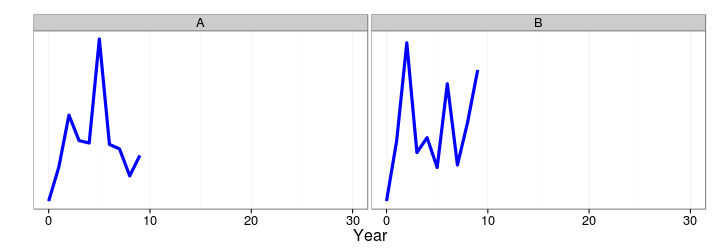
\includegraphics[height=25mm,width=100mm]{doug5.png}\end{frame}
%\begin{frame}\frametitle{MSE Example} \smallskip\textbf{There has been a {\color{blue} Regime Shift}}\smallskip\\ Is it A or B? 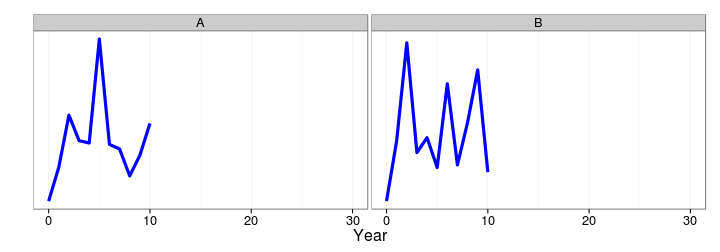
\includegraphics[height=25mm,width=100mm]{doug6.png}\end{frame}
\begin{frame}\frametitle{MSE Example} \smallskip\textbf{There has been a {\color{blue} Regime Shift}}\smallskip\\ Is it A or B? 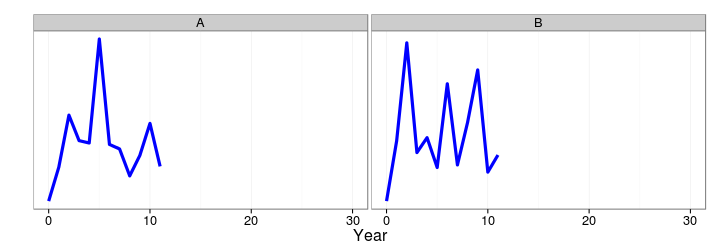
\includegraphics[height=25mm,width=100mm]{doug7.png}\end{frame}
%\begin{frame}\frametitle{MSE Example} \smallskip\textbf{There has been a {\color{blue} Regime Shift}}\smallskip\\ Is it A or B? 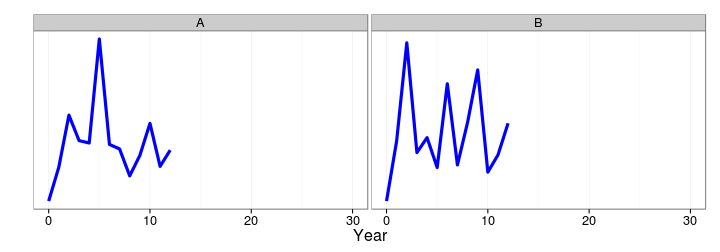
\includegraphics[height=25mm,width=100mm]{doug8.png}\end{frame}
%\begin{frame}\frametitle{MSE Example} \smallskip\textbf{There has been a {\color{blue} Regime Shift}}\smallskip\\ Is it A or B? 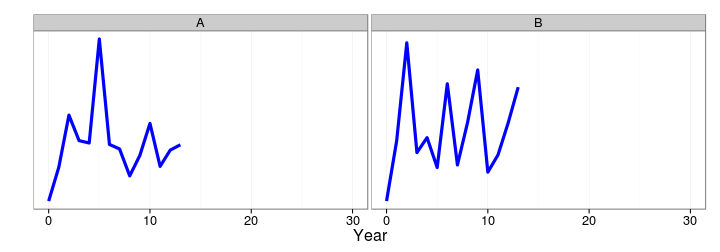
\includegraphics[height=25mm,width=100mm]{doug9.png}\end{frame}
\begin{frame}\frametitle{MSE Example} \smallskip\textbf{There has been a {\color{blue} Regime Shift}}\smallskip\\ Is it A or B? 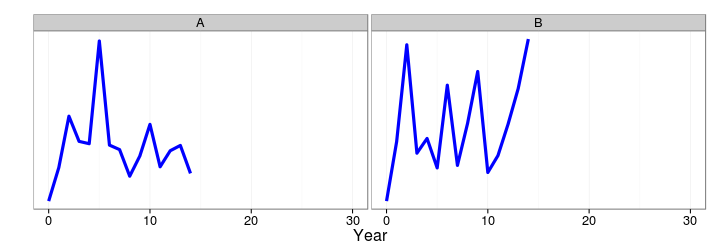
\includegraphics[height=25mm,width=100mm]{doug10.png}\end{frame}
%\begin{frame}\frametitle{MSE Example} \smallskip\textbf{There has been a {\color{blue} Regime Shift}}\smallskip\\ Is it A or B? 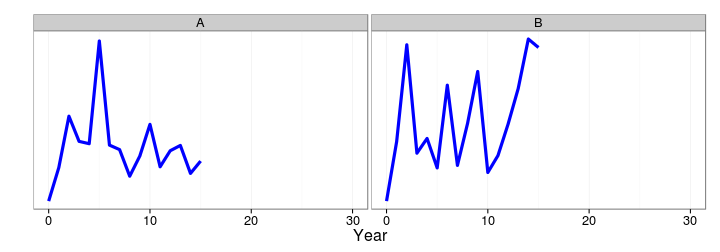
\includegraphics[height=25mm,width=100mm]{doug11.png}\end{frame}
%\begin{frame}\frametitle{MSE Example} \smallskip\textbf{There has been a {\color{blue} Regime Shift}}\smallskip\\ Is it A or B? 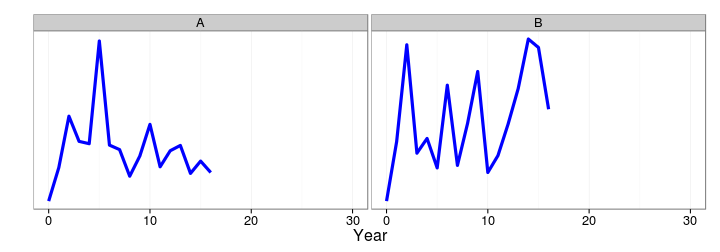
\includegraphics[height=25mm,width=100mm]{doug12.png}\end{frame}
\begin{frame}\frametitle{MSE Example} \smallskip\textbf{There has been a {\color{blue} Regime Shift}}\smallskip\\ Is it A or B? 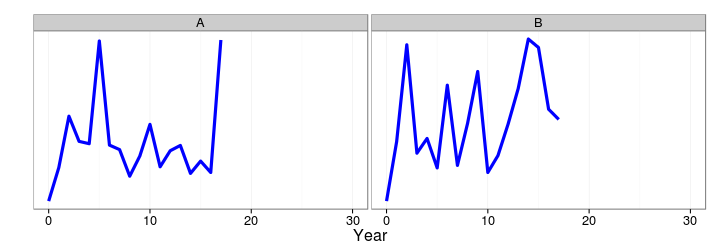
\includegraphics[height=25mm,width=100mm]{doug13.png}\end{frame}
%\begin{frame}\frametitle{MSE Example} \smallskip\textbf{There has been a {\color{blue} Regime Shift}}\smallskip\\ Is it A or B? 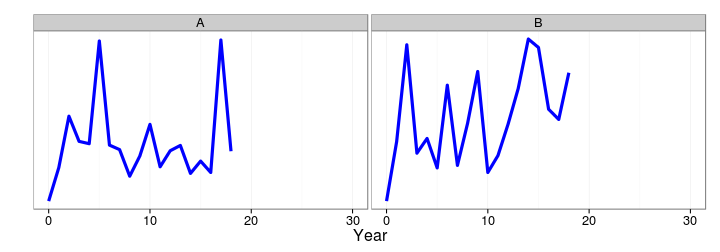
\includegraphics[height=25mm,width=100mm]{doug14.png}\end{frame}
%\begin{frame}\frametitle{MSE Example} \smallskip\textbf{There has been a {\color{blue} Regime Shift}}\smallskip\\ Is it A or B? 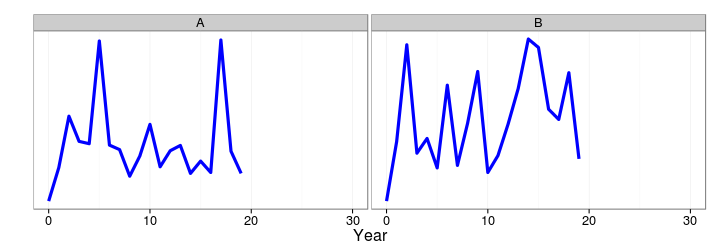
\includegraphics[height=25mm,width=100mm]{doug15.png}\end{frame}
\begin{frame}\frametitle{MSE Example} \smallskip\textbf{There has been a {\color{blue} Regime Shift}}\smallskip\\ Is it A or B? 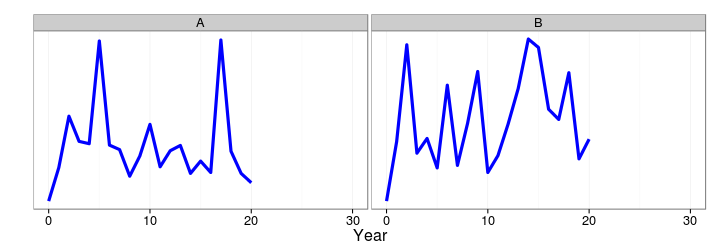
\includegraphics[height=25mm,width=100mm]{doug16.png}\end{frame}
%\begin{frame}\frametitle{MSE Example} \smallskip\textbf{There has been a {\color{blue} Regime Shift}}\smallskip\\ Is it A or B? 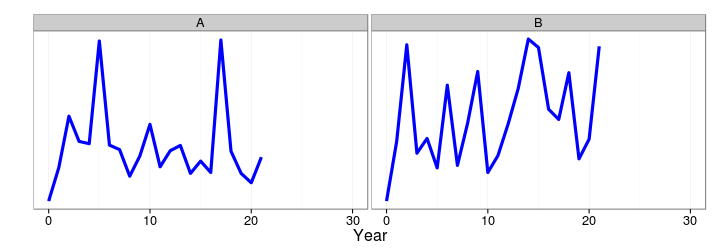
\includegraphics[height=25mm,width=100mm]{doug17.png}\end{frame}
%\begin{frame}\frametitle{MSE Example} \smallskip\textbf{There has been a {\color{blue} Regime Shift}}\smallskip\\ Is it A or B? 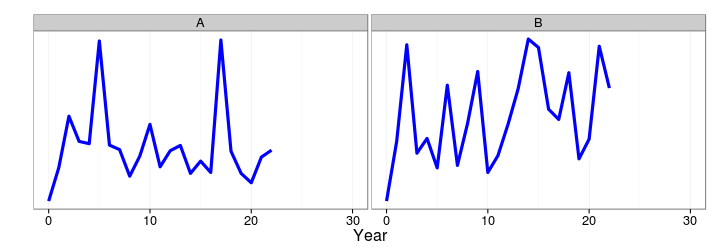
\includegraphics[height=25mm,width=100mm]{doug18.png}\end{frame}
\begin{frame}\frametitle{MSE Example} \smallskip\textbf{There has been a {\color{blue} Regime Shift}}\smallskip\\ Is it A or B? 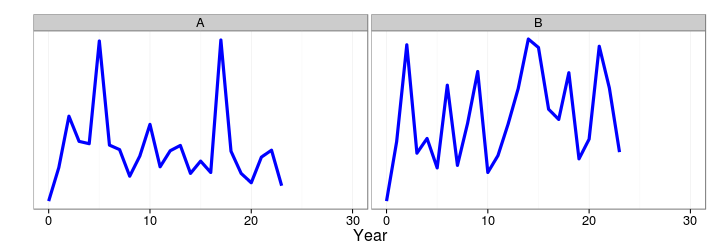
\includegraphics[height=25mm,width=100mm]{doug19.png}\end{frame}
%\begin{frame}\frametitle{MSE Example} \smallskip\textbf{There has been a {\color{blue} Regime Shift}}\smallskip\\ Is it A or B? 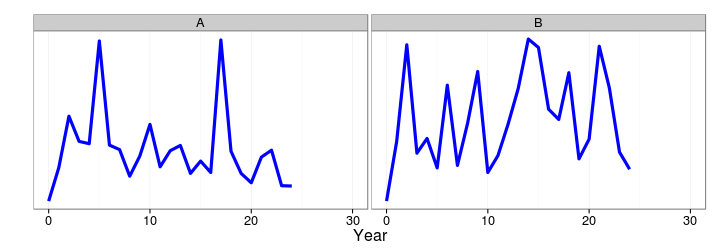
\includegraphics[height=25mm,width=100mm]{doug20.png}\end{frame}
%\begin{frame}\frametitle{MSE Example} \smallskip\textbf{There has been a {\color{blue} Regime Shift}}\smallskip\\ Is it A or B? \includegraphics[height=25mm,width=100mm]{doug21.png}\end{frame}
\begin{frame}\frametitle{MSE Example} \smallskip\textbf{There has been a {\color{blue} Regime Shift}}\smallskip\\ Is it A or B? \includegraphics[height=25mm,width=100mm]{doug22.png}\end{frame}
%\begin{frame}\frametitle{MSE Example} \smallskip\textbf{There has been a {\color{blue} Regime Shift}}\smallskip\\ Is it A or B? \includegraphics[height=25mm,width=100mm]{doug23.png}\end{frame}
%\begin{frame}\frametitle{MSE Example} \smallskip\textbf{There has been a {\color{blue} Regime Shift}}\smallskip\\ Is it A or B? \includegraphics[height=25mm,width=100mm]{doug24.png}\end{frame}
\begin{frame}\frametitle{MSE Example} \smallskip\textbf{There has been a {\color{blue} Regime Shift}}\smallskip\\ Is it A or B? \includegraphics[height=25mm,width=100mm]{doug25.png}\end{frame}
%\begin{frame}\frametitle{MSE Example} \smallskip\textbf{There has been a {\color{blue} Regime Shift}}\smallskip\\ Is it A or B? \includegraphics[height=25mm,width=100mm]{doug26.png}\end{frame}
\begin{frame}\frametitle{MSE Example} \smallskip\textbf{There has been a {\color{blue} Regime Shift}}\smallskip\\ \textbf{It was A} \includegraphics[height=25mm,width=100mm]{doug27.png}\end{frame}
\begin{frame}\frametitle{MSE Example} \smallskip\textbf{There has been a {\color{blue} Regime Shift}}\smallskip\\ \textbf{It was A, {\color{red} but it took 20 years to work it out!}} \includegraphics[height=25mm,width=100mm]{doug27.png}\end{frame}

\begin{frame}{MSE Example}
     %\smallskip\textbf{MSE Example}\smallskip\\
     \begin{columns}[t] 
     \begin{column}[T]{5cm} 
        \smallskip It took 20 years to work out that the stock had experienced a decline unrelated to fishing\smallskip\\
     \textbf{{\color{red} But we can not wait 20 years!}}
     \end{column}
     \begin{column}[T]{5cm}
      \smallskip\textbf{What to do?} run an MSE\smallskip\\
       \Fontviii
       \begin{itemize}[<+->]
          \item Simulate two hypotheses, i.e.
          \begin{itemize}
	    \Fontvi
            \item No Change  or 
	    \item Change in Productivity.
          \end{itemize}
          \item Evaluate alternative management strategies i.e.
          \begin{itemize}
	    \Fontvi
	    \item \textbf{I} Constant Catch
	    \item \textbf{II} 5\% of Assessed Stock Biomass
	    \item \textbf{III} 80\% of Last Years Catch + 20\% of Catch under II
	  \end{itemize}
       \end{itemize}
     \end{column}
    \end{columns}    
\end{frame}

\begin{frame}\frametitle{MSE Example}
\smallskip\textbf{Which Strategy is most robust}\smallskip\\
\begin{columns}[t] 
\begin{column}[T]{4cm} % each column can also be its own environment
     \smallskip\textbf{Strategies}\smallskip\\
       \Fontviii
       \begin{itemize}
          \item \textbf{I} Constant catch
          \item \textbf{II} 5\% of Assessed stock biomass
          \item \textbf{III} 80\% of last years catch + 20\% of catch given under II
        \end{itemize}
     \end{column}
\begin{column}[T]{6cm}
 \smallskip\textbf{What are the yields like?}\smallskip\\ 
  \includegraphics[height=48mm,width=64mm]{mp2.png}
\end{column}
     \end{columns}    
\end{frame}

\begin{frame}\frametitle{MSE Example}
\smallskip\textbf{Which Strategy is most robust}\smallskip\\
\begin{columns}[t] 
\begin{column}[T]{4cm} % each column can also be its own environment
     \smallskip\textbf{Strategies}\smallskip\\
       \Fontviii
       \begin{itemize}
          \item \textbf{I} Constant catch
          \item \textbf{II} 5\% of Assessed stock biomass
          \item \textbf{III} 80\% of last years catch + 20\% of catch given under II
        \end{itemize}
     \end{column}
\begin{column}[T]{6cm}
 \smallskip\textbf{What happened to the Stock?}\smallskip\\ 
  \includegraphics[height=48mm,width=64mm]{mp1.png}
\end{column}
\end{columns}    
\end{frame}


\begin{frame}\frametitle{MSE Example}
\smallskip\textbf{Run more simulations to look at variability}\smallskip\\
\begin{columns}[t] 
\begin{column}[T]{4cm} % each column can also be its own environment
     \smallskip\textbf{Strategies}\smallskip\\
       \Fontviii
       \begin{itemize}
          \item \textbf{I} Constant catch
          \item \textbf{II} 5\% of Assessed stock biomass
          \item \textbf{III} 80\% of last years catch + 20\% of catch given under II
        \end{itemize}
     \smallskip\textbf{Results}\smallskip\\
       \Fontviii
       \begin{itemize}
          \item Catch most variable under \textbf{II}
        \end{itemize}
     \end{column}
\begin{column}[T]{6cm}
 \smallskip\textbf{What are the yields like?}\smallskip\\ 
  \includegraphics[height=48mm,width=64mm]{mp6.png}
\end{column}
     \end{columns}    
\end{frame}

\begin{frame}\frametitle{MSE Example}
\smallskip\textbf{Run more simulations to look at variability}\smallskip\\
\begin{columns}[t] 
\begin{column}[T]{4cm} % each column can also be its own environment
     \smallskip\textbf{Strategies}\smallskip\\
       \Fontviii
       \begin{itemize}
          \item \textbf{I} Constant catch
          \item \textbf{II} 5\% of Assessed stock biomass
          \item \textbf{III} 80\% of last years catch + 20\% of catch given under II
        \end{itemize}
     \smallskip\textbf{Results}\smallskip\\
       \Fontviii
       \begin{itemize}
          \item \textbf{I} and \textbf{II} are robust
        \end{itemize}
     \end{column}
 \begin{column}[T]{6cm}
 \smallskip\textbf{What happened to the Stock?}\smallskip\\ 
  \includegraphics[height=48mm,width=64mm]{mp5.png}
\end{column}
    \end{columns}    
\end{frame}

\begin{frame}\frametitle{MSE Example}
\smallskip\textbf{Results from MSE}\smallskip\\
       \begin{itemize}[<+->]
          \Fontviii
          \item Strategies \textbf{II} and \textbf{III} are robust
          \item Catch is more variable under Strategy \textbf{II}
          \item Risk of not being in the Green Quadrant?
          \item Trade-offs between objectives?
          \item Risk of SCRS getting dynamics wrong and {\color{blue} Regime Shifts}, ...
          \item How to prioritise funding to get appropriate research, monitoring and enforcement levels? \textbf{Josu made me add this!}
        \end{itemize}
\end{frame}

%\begin{frame}\frametitle{MSE Example} \smallskip\textbf{What happens to the Stock?}\smallskip\\ \includegraphics[height=48mm,width=64mm]{mp1.png}\end{frame}
%\begin{frame}\frametitle{MSE Example} \smallskip\textbf{Example}\smallskip\\ \includegraphics[height=48mm,width=64mm]{mp3.png}\end{frame}
%\begin{frame}\frametitle{MSE Example} \smallskip\textbf{Example}\smallskip\\ \includegraphics[height=48mm,width=64mm]{mp4.png}\end{frame}
%\begin{frame}\frametitle{MSE Example} \smallskip\textbf{What are the yields like?}\smallskip\\ \includegraphics[height=48mm,width=64mm]{mp6.png}\end{frame}
%\begin{frame}\frametitle{MSE Example} \smallskip\textbf{What happens to the Stock?}\smallskip\\ \includegraphics[height=48mm,width=64mm]{mp5.png}\end{frame}


%\begin{frame}\frametitle{Management Procedures} \smallskip\textbf{Example}\smallskip\\ \includegraphics[]{scen.png}\end{frame}
%\begin{frame}\frametitle{Management Procedures} \smallskip\textbf{Example}\smallskip\\ \includegraphics[]{scen2.png}\end{frame}

\begin{frame}{Conditioning Operating Models}
  \smallskip\textbf{Stock Assessment}\smallskip\\
  \begin{columns}[t] % contents are top vertically aligned
   \begin{column}[T]{5cm} % alternative top-align that's better for graphics
    \includegraphics[height=40mm]{kobePlot-swon.png}
   \end{column}
   \begin{column}[T]{6cm} % each column can also be its own environment
   \Fontviii
   \textbf{Scenarios}
   \begin{itemize}%[<+->]
       \item {\color{blue} North Atlantic Swordfish:} \textbf{1 Assessment}
       \item {\color{blue} North Atlantic Albacore:} \textbf{7 Assessments} Alternative CPUE Indices
       \item {\color{blue} Mediterranean Bluefin Tuna:} \textbf{6 Assessments} 2 sets of Historical Catch and 3 Future Recruitment Levels 
   \end{itemize}
   \end{column}
\end{columns}
\end{frame}

\begin{frame}{Conditioning Operating Models}
  \smallskip\textbf{Running an MSE requires many Operating Models}\smallskip\\
  \begin{columns}[t] % contents are top vertically aligned
 % \smallskip\textbf{North Atlantic Swordfish}\smallskip\\
   \begin{column}[T]{5cm} % alternative top-align that's better for graphics
    \includegraphics[height=40mm]{kobeGrid.png}
   \end{column}
   \begin{column}[T]{5cm} % each column can also be its own environment
   \Fontviii
   \smallskip\textbf{Many more hypotheses to be considered}\smallskip\\
   \begin{itemize}%[<+->]
       \item {\color{blue} Task I \& II:} Quqlity of data
       \item {\color{blue} Cpue Indices:}
       \item {\color{blue} Choice of Reference Points:}
       \item {\color{blue} M:} Knowledge of biology
       \item {\color{blue} Ageing:} Data processing
       
       \item {\color{blue} ...}
   \end{itemize}
   \end{column}
\end{columns}
\end{frame}


\begin{frame}{MSE Work By SCRS}
   \smallskip\textbf{MSE Work In Progress}\smallskip\\
   \Fontviii
   \begin{description}%[<+->]
       \item[Generic] \textbf{Operating Model} based either on an existing stock assessment,  e.g. North Atlantic Albacore, or life history characteristics for data poor stocks. \\ 
       \textbf{Management Procedure} a biomass stock assessment model using only CPUE and catch, e.g. North Atlantic Swordfish.
       \item[GBYP] \textbf{Management Procedures} based on an stock assessment models or data only (e.g. Southern Bluefin).\\
       \textbf{Operating Model} includes a range of hypotheses and will simulate data sets to reflect uncertainty about knowledge of biology, ecology and our ability to observe and control the fisheries. \\ 
       \textbf{Evaluation} with respect to their ability to meet multiple management objectives and trade-offs between them for different choices e.g.
       to invest in surveys, tagging, biological studies, more monitoring, better control, ...
    \end{description}
\end{frame}

\begin{frame}\frametitle{Six Step Process for Conducting an MSE} 
  \smallskip\textbf{Six Step Program}\smallskip
  \Fontviii
  \begin{description}%[<+->]
    \item[Identification] of management objectives and mapping these to performance measures to quantify how well they are achieved\
    \item[Selection] of hypotheses about system dynamics for building \textbf{O}perating \textbf{M}odels (i.e. Simulation Models)
    \item[Building] the simulation models, i.e. Conditioning the OMs on data and knowledge, and possible rejection of and weighting of the different hypotheses.
    \item[Identifying] alternative management strategies, i.e.the combination of pre-defined data, stock assessment methods and reference points and HCRs.
    \item[Running] the simulations using the HCRs as feedback control procedures; and
    \item[Agreeing] the Management Strategies that best meet management objectives.
 \end{description}
 \end{frame}


\begin{frame}\frametitle{Management Strategy Evaluation} 
  \smallskip\textbf{Use of simulation modelling to evaluate the impact of the main sources of uncertainties}\smallskip 
  \Fontviii
  \begin{itemize} %[<+->]
     \item Allows a fuller consideration of uncertainty as required by the Precautionary Approach; 
     \item Provides stability if management objectives and how to evaluate how well alternative  
	   management strategies meet them are agreed through a dialogue between scientists and stakeholders; and 
     \item Can be used to guide the scientific process by identifying where the reduction of scientific 
	   uncertainty will improve management and so help to ensure that expenditure is prioritised to provide 
	   the best research, monitoring and enforcement. 
  \end{itemize}
\end{frame}

\end{document}


\begin{frame}
\frametitle{Quantitative uncertainties: the ``grid''}
\begin{itemize}
    \item Key parameters/options where may not have convincing information in data \emph{but} can explore quantitative options:
        \begin{enumerate}
            \item {\color{orange} Steepness (h)}: strong but one-way trip decline in CPUE...
            \item {\color{orange}$M_{0,10}$}: no direct data but vital to define shape of $M_a$
            \item {\color{orange} $\omega$}: non-linearity of biomass-to-CPUE relationship
            \item {\color{orange} CPUE series}: spatial weighting options for core series
            \item {\color{orange} $q$ age-range}: ages over which LL CPUE $q$ calculated
            \item {\color{orange} Sample size}: initial effective sample sizes 
        \end{enumerate}
    \item With grid elements have pre-defined priors \emph{but} option of resampling based on objective function
\end{itemize}
\end{frame}


\begin{frame}
\frametitle{Quantitative uncertainties: the ``grid''}
\begin{itemize}
    \item For MSE work grid option table (reference set of OMs):
\begin{table}
\begin{center}
\label{tab:datasumm}
\begin{tabular}{|cccccc|}
\hline
& {\tiny Levels} & {\tiny CumulN} & {\tiny Values} & {\tiny Prior} & {\tiny Weighting}\\
\hline\hline
{\tiny $h$} & {\tiny 5} & {\tiny 5} & {\tiny 0.55, 0.64, 0.93, 0.82, 0.9} & {\tiny uniform} & {\tiny obj. fun.}\\
{\tiny $M_0$} & {\tiny 4} & {\tiny 20} & {\tiny 0.3, 0.35, 0.4, 0.45} & {\tiny uniform} & {\tiny obj. fun.}\\
{\tiny $M_{10}$} & {\tiny 3} & {\tiny 60} & {\tiny 0.07, 0.1, 0.14} & {\tiny uniform} & {\tiny obj. fun.}\\
{\tiny $\omega$} & {\tiny 1} & {\tiny 60} & {\tiny 1} & {\tiny NA} & {\tiny NA}\\
{\tiny CPUE} & {\tiny 2} & {\tiny 120} & {\tiny w.5, w.8} & {\tiny uniform} & {\tiny prior}\\
{\tiny $q$ age-range} & {\tiny 2} & {\tiny 240} & {\tiny 4-18, 8-12} & {\tiny 0.67, 0.33} & {\tiny prior}\\
{\tiny Sample size} & {\tiny 1} & {\tiny 240} & {\tiny SQRT} & {\tiny NA} & {\tiny NA}\\
\hline
\end{tabular}
\end{center}
\end{table}
\item From 240 grid permutations sample of 2000 generated
\end{itemize}
\end{frame}


\subsection{Management objectives}
\begin{frame}\frametitle{Kobe} 
 \Fontviii
  \smallskip\textbf{Biological advice used by ICCAT is based upon which quadrant a stock falls into}\smallskip
\begin{description}%[<+->]
 \item[Green:] stock is neither overfished nor subject to overfishing, management shall 
 result in a high probability of maintaining the stock within this quadrant.
 \item[Red:] stock is overfished and subject to overfishing,
  the Commission shall immediately adopt management measures, taking into account, inter alia, the biology
 of the stock and SCRS advice, designed to result in a high probability of ending overfishing in as short a
period as possible. In addition, the Commission shall adopt a plan to rebuild these stocks taking into
account, inter alia, the biology of the stock and SCRS advice.
 \item[Upper Right Yellow:] stock is not overfished but subject to overfishing, the Commission shall 
immediately adopt management measures, taking into
 account, inter alia, the biology of the stock and SCRS advice, designed to result in a high probability of
ending overfishing in as short a period as possible.
 \item[Lower Left Yellow:] stock is overfished but not subject to overfishing, the Commission shall 
 adopt management measures designed to rebuild these stocks in as
 short a period as possible, taking into account, inter alia, the biology of the stock and SCRS advice.  
\end{description}
\end{frame}

\subsection{Conditioning}
There will always be alternative aims for constructing operating model to evaluate MPs, which may include the following, although the list is not attempted to be exhaustive. 
The operating model corresponds to one of the following.
(1) The currently used assessment model, this implies that assessment models describe nature almost perfectly.
(2) Best fit to all available and justified data (in Bayesian models priors would be non-informative, i.e. only data would “speak”). This approach is based on the idea that all relevant data sets are available and that data is the only thing that matters when considering future events.
(3) Best description of all available information in relation to the fitting of historic data (in Bayesian models priors would describe in a formal way the knowledge of scientists related to the validity of information sources). It is believed that the future will be like the past with no information to the contrary. Probabilities, other than those available from data, may come from, for example a meta-analysis.
(4) Best prediction of the future dynamics, given the historic data. In this case, the emphasis is on expert beliefs and other such prior type information about future processes being relevant when testing the behaviour of management systems in the future (i.e. the focus is on the future, not on fitting historic data). For example, climatic change studies may show that a regime shift is likely and should be taken into account when providing future advice. This was the case in the Baltic, where high precipitation has impacted various stocks, and this change was predicted before fisheries scientists could provide low enough p-values from their data sets. It is important therefore that operational models are flexible, so that they can deal with such aspects. The use of priors in the operational model would offer a flexible way to deal with these various elements. 
It may be considered, that (4) is related to the testing of the robustness of MPs to alternative hypothesis about the dynamics and that (2) represents the base case. As the aim of the OM modelling is to test different types of plausible hypothesis in a management framework, type (3) and (4) models are most important types after the base case is agreed.

\subsection{Commission}

12. Identification of matters for presentation to and consideration by the Commission, including any recommendations as well as proposed next steps for SWGSM 

There was broad agreement that the first meeting of the Working Group was very successful and the SWGSM made the following recommendations. There should be another meeting of the Working Group in 2015. On the issue of the possible subject matters to be discussed at the next meeting, many delegations were of the view that it would be useful to proceed with practical examples that could help advance the dialogue for individual stocks. However, it was also suggested that dialogue of a general nature continue on issues such as acceptable levels of risk, targets, limits and time horizons. Noting the low participation, it was recommended that the Commission consider providing funds for two members per delegation (one manager and one scientist) for those CPCs needing assistance. It was also suggested that the next meeting should have greater balance in the numbers of participating scientists and managers. 

The SWGSM agreed that skipjack, which will be assessed in 2014, would be a good candidate to examine harvest control rules for a stock that is in a healthy status. North Atlantic albacore and North Atlantic swordfish, stocks for which the SCRS has already advanced HCR development and testing, were also considered as good candidates. Many delegations also proposed that Atlantic bluefin tuna be considered as a priority species and the working group recommended that it be discussed at the next meeting. The management of this species has required substantial quota reductions and fishery indicators suggest that it is rapidly recovering. For this reason, the development of a HCR for bluefin is needed so that future TAC adjustments can be made in a reliable and defensible fashion. In order to eliminate data gaps that affect the timeliness of stock assessments, it would be important to also consider improvements in fishery monitoring, including real-time reporting. 

